The aim of this chapter is to review

%%%%%%%%%%%%%%%%%%%%%%%%%%%%%%%%%%%%%%%%%%%%%%%%%%%%%%%%%%%%%%%%%%%%
%%%%%%%%%%%%%%%%%%%%%%%%%%%%%%%%%%%%%%%%%%%%%%%%%%%%%%%%%%%%%%%%%%%%
%%%%%%%%%%%%%%%%%%%%%%%%%%%%%%%%%%%%%%%%%%%%%%%%%%%%%%%%%%%%%%%%%%%%

\section{Testing Data}

\subsection{Database Videos}

The system is tested using a database of 50 different videos, ranging from 7 to 14 seconds, as per requirements F25-F26. The database of videos is populated from scratch using free stock footage from \textit{Pexels Video}\footnote{Pexels Video: \url{https://www.pexels.com/videos/}}. The videos used to build the database are chosen from a rich library of videos encapsulating many different colours (e.g. bright, dark, warm, cold, colourful, etc.) and movements (e.g. still, motion, shaky, blurry, timelapses, etc.) to ensure diversification. The database of videos used to test the system can be found in the \textit{``footage''} directory in the provided code.\\

Employing existing databases of videos for CBVR tasks such as the TRECVID\footnote{Text REtrieval Conference Video Retrieval Evaluation} dataset \cite{2018trecvidawad}, which is the best dataset for CBVR-oriented tasks, would have been ideal to measure the project's performance and to compare it with existing solutions for this task. However, these datasets are not publicly available and hard to obtain. For example, most of the referenced papers in the Bibliography that present CBVR solutions were conducted for the TRECVID conferences, meaning that the datasets were provided to the participants for testing and evaluating results. However, the NIST\footnote{National Institute of Standards and Technology, organiser of the annual TRECVID conference} does not provide these databases for external papers. Other databases of videos exist, but target other computer vision tasks such as facial recognition or image retrieval rather than CBVR. Therefore, the previously mentioned custom database of 50 videos is used to test this system.\\

%%%%%%%%%%%%%%%%%%%%%%%%%%%%%%%%%%%%%%%%%%%%%%%%%%%%%%%%%%%%%%%%%%%%

\subsection{Query Videos}

Various query videos are recorded to test the online retrieval phase of the system. These queries are mobile recordings of one of the database videos. Different types of queries listed in Section \ref{sec:design-query-video-processing} are used to test the limits of the system, including down-scaled (recording at a distance from the screen) and skewed queries (recording at an angle) coupled with minor camera movement due to shaking hands. These conditions ensure the realism of the queries if the system were to be developed as a mobile application.

%%%%%%%%%%%%%%%%%%%%%%%%%%%%%%%%%%%%%%%%%%%%%%%%%%%%%%%%%%%%%%%%%%%%
%%%%%%%%%%%%%%%%%%%%%%%%%%%%%%%%%%%%%%%%%%%%%%%%%%%%%%%%%%%%%%%%%%%%
%%%%%%%%%%%%%%%%%%%%%%%%%%%%%%%%%%%%%%%%%%%%%%%%%%%%%%%%%%%%%%%%%%%%

\section{Results Analysis}

The results are evaluated by counting the number of true positives and false positives for each video query used to test the system. A true positive corresponds to an outcome where the system matches the query to the correct database video, while a false positive is an outcome where the system matches the query incorrect to an incorrect database videos. The number of true positives and false positives occurrences are counted for each histogram model and distance metric used per query. As detailed in the previous chapter at the end of Section \ref{sec:implementation-distance-measurements}, these are used to plot the probabilities of the most likely database video to match the query in the form of a percentage \%. Additionally, other measurements are made such as the runtime of the system, its scalability, and the comparison of the final results under different conditions.\\

Before analysing the main result of the online retrieval phase where queries are matched to a database video, the offline colour-based feature extraction phase is first briefly analysed.

%%%%%%%%%%%%%%%%%%%%%%%%%%%%%%%%%%%%%%%%%%%%%%%%%%%%%%%%%%%%%%%%%%%%

\subsection{Offline Colour-Based Feature Extraction Phase Runtime}

todo, mention runtime and scalability

%%%%%%%%%%%%%%%%%%%%%%%%%%%%%%%%%%%%%%%%%%%%%%%%%%%%%%%%%%%%%%%%%%%%

\subsection{Online Retrieval}

\subsubsection{Accuracy}

The system is first tested with down-scaled queries recorded at a straight angle to the screen. Shaky camera movement can be seen on the query videos, along with a lot of frame area not covering the actual database video playing due to the distance to the screen. Despite these challenges, the queries still yield high accuracy exceeding 50\% true positives, with some excellent results that exceed 90\%. Recs 1 and 2.

\begin{figure}[h] 
\centerline{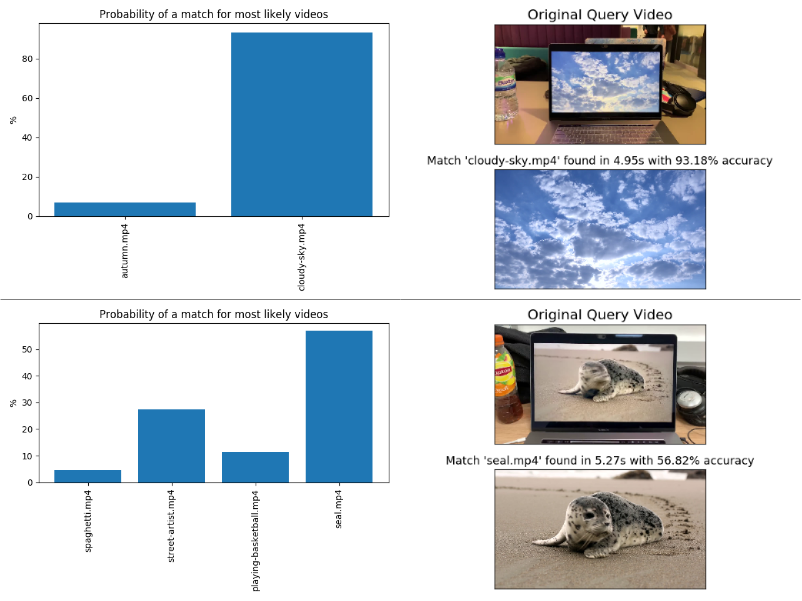
\includegraphics[width=\textwidth]{figures/evaluation/downscaled-queries.png}}
\caption{\label{fig:evaluation-downscaled-queries}Down-scaled Queries.}
\end{figure}

Next, skewed queries recorded at an angle from the screen playing the database video are tested. These also included all of the challenges mentioned in the first test, such as down-scaling and unstable footage. The accuracy of the matches still exceed 50\% and reach as high as 75\% despite the added poor quality factor of the query video. recs 3 and 8.

\begin{figure}[h] 
\centerline{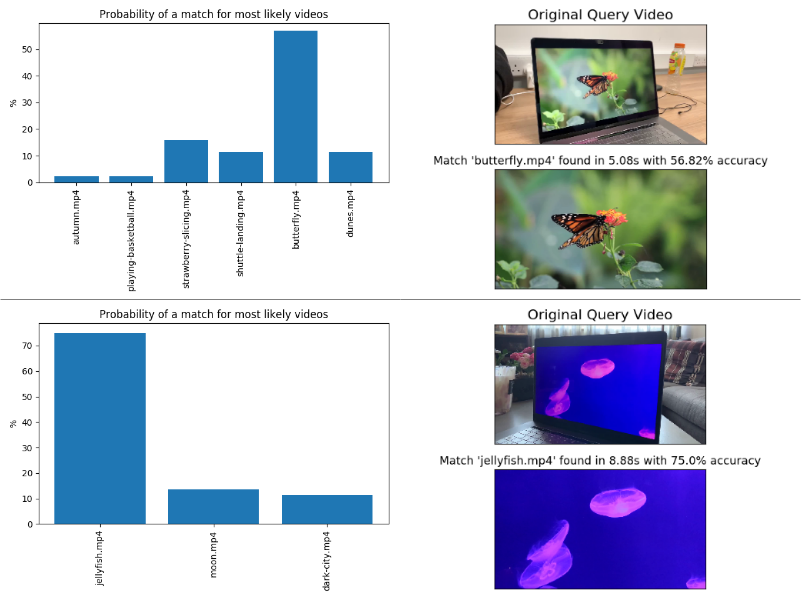
\includegraphics[width=\textwidth]{figures/evaluation/skewed-queries.png}}
\caption{\label{fig:evaluation-skewed-queries}Skewed Queries.}
\end{figure}

However, despite the good results portrayed in the first two tests, some queries yield poor accuracy for some matches as low as 45.5\%. This may be due to a number of factors that are further explored in Section \ref{sec:evaluation-observations-online-phase} with more examples.(use rec5)\\

\begin{figure}[h] 
\centerline{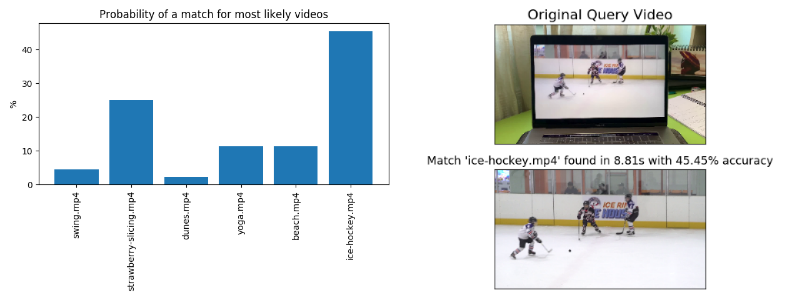
\includegraphics[width=\textwidth]{figures/evaluation/poor-accuracy-query.png}}
\caption{\label{fig:evaluation-poor-accuracy-query}Poor accuracy Query.}
\end{figure}

\subsubsection{Runtime}

Requirement F13

\begin{figure}[h] 
\centerline{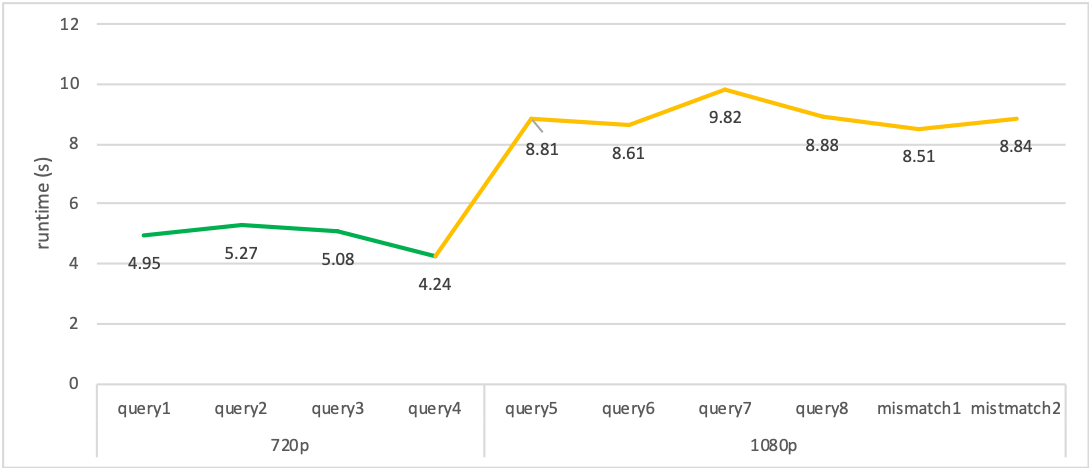
\includegraphics[width=\textwidth]{figures/evaluation/runtime_plot.png}}
\caption{\label{fig:evaluation-runtime_plot}Runtime plot.}
\end{figure}

\subsection{Observations}
\label{sec:evaluation-observations-online-phase}

As mentioned in the previous paragraph, external factors affecting the quality of the query can drastically affect the accuracy of the system, and even produce wrong matches. The first noticeable condition that causes the system to produce low-accuracy results or wrong matches is the lighting in the room. When recording query videos during night-time with lamps that produce warm white light (colour temperatures ranging between 2000K and 3000K)\footnote{What is colour temperature? \url{http://www.westinghouselighting.com/color-temperature.aspx}}, which corresponds to orange/yellow light, the overall colour of the recorded screen changes. This causes the system to have trouble matching the query video's histograms to the correct database videos' histograms. (use rec4 and failed butterfly recording)

\begin{figure}[h] 
\centerline{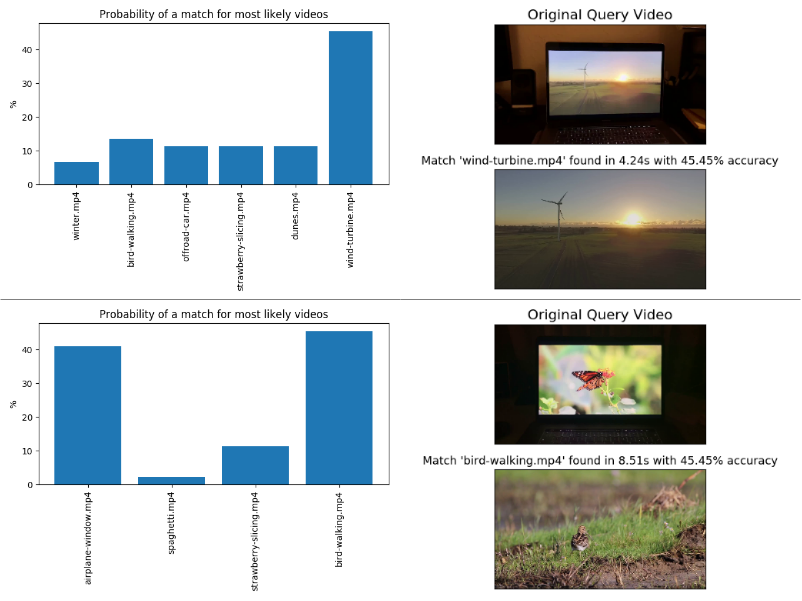
\includegraphics[width=\textwidth]{figures/evaluation/yellow-light-queries.png}}
\caption{\label{fig:evaluation-yellow-light-queries}Yellow light Queries.}
\end{figure}

\begin{comment}
pixel intensity in dark room with 

general observation: lighting affecting system accuracy (at night time, in dark room with small lamps that produce yellow light)
\end{comment}

Another external factor is the presence of light reflections on the screen displaying the database videos. Depending on the positioning of the light source and the camera recording the query, light glares might appear on the screen, greatly affecting the accuracy of the system as new colours appear on the screen, causing the histograms' pixel intensities to converge towards that new colour. (example failed spaghetti recording and rec7)

\begin{figure}[h] 
\centerline{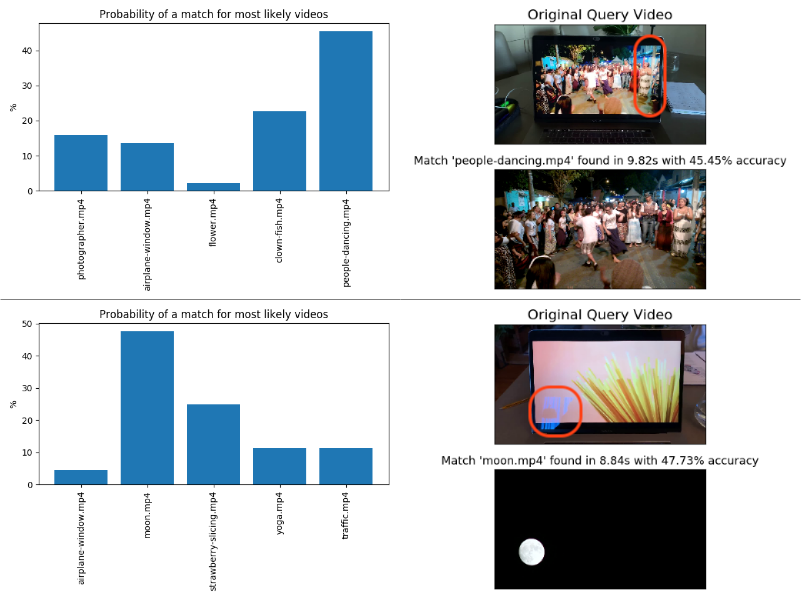
\includegraphics[width=\textwidth]{figures/evaluation/light-reflection-queries.png}}
\caption{\label{fig:evaluation-light-reflection-queries}Light Reflection Queries.}
\end{figure}

%%%%%%%%%%%%%%%%%%%%%%%%%%%%%%%%%%%%%%%%%%%%%%%%%%%%%%%%%%%%%%%%%%%%
%%%%%%%%%%%%%%%%%%%%%%%%%%%%%%%%%%%%%%%%%%%%%%%%%%%%%%%%%%%%%%%%%%%%
%%%%%%%%%%%%%%%%%%%%%%%%%%%%%%%%%%%%%%%%%%%%%%%%%%%%%%%%%%%%%%%%%%%%

\section{Histogram Models and Distance Metrics Performance Analysis}

analyse results of RGB, grey scale and HSV histograms with the 6 different histogram matching methods. which work best? in which scenarios? (use the 10 previous results to show this)

removing KL divergence metric greatly improved accuracy. (using less metric to use the ones for the job). KL divergence NEVER found correct match, not meant to be used a distance metric (show example of removing KL div and alternate chi square with past examples and new one)

improved cloudy-sky,
improved butterfly skewed

%%%%%%%%%%%%%%%%%%%%%%%%%%%%%%%%%%%%%%%%%%%%%%%%%%%%%%%%%%%%%%%%%%%%
%%%%%%%%%%%%%%%%%%%%%%%%%%%%%%%%%%%%%%%%%%%%%%%%%%%%%%%%%%%%%%%%%%%%
%%%%%%%%%%%%%%%%%%%%%%%%%%%%%%%%%%%%%%%%%%%%%%%%%%%%%%%%%%%%%%%%%%%%

\section{Comparison With Ground Truth Experiment}

online classification experiment:
    \begin{itemize}
        \item Google Survey experiment results 
        \item Compare experiment results with the algorithm results
        \item use a plot to visualise experiment results
        \item link to appendix (Ethics Checklist Appendix \ref{ch:appendix-ethics-checklist}, Experiment Script Appendix \ref{ch:appendix-experiment-survey}, and Raw Results)
    \end{itemize}
    
mention ground truth (https://en.wikipedia.org/wiki/Ground\_truth) (https://www.techopedia.com/definition/32514/ground-truth)

%%%%%%%%%%%%%%%%%%%%%%%%%%%%%%%%%%%%%%%%%%%%%%%%%%%%%%%%%%%%%%%%%%%%
%%%%%%%%%%%%%%%%%%%%%%%%%%%%%%%%%%%%%%%%%%%%%%%%%%%%%%%%%%%%%%%%%%%%
%%%%%%%%%%%%%%%%%%%%%%%%%%%%%%%%%%%%%%%%%%%%%%%%%%%%%%%%%%%%%%%%%%%%

\section{Database Pre-Processing Test: Movie Segmentation}

The shot boundary detection algorithm is used on a feature-length movie. The movie used for the test is Inception\footnote{Inception IMDb page: https://www.imdb.com/title/tt1375666/}. The movie is composed of 213098 frames.

The shot boundary detection algorithm is used once with the KL Divergence and once with the Intersection metric..

\begin{itemize}
    \item KL Divergence: a global threshold of 10 using the KL Divergence detects 661 shot boundaries (0,31\%) in 149.7 minutes.
    \item Intersection: A global threshold of 7 using the Intersection metric detects 1730 shot boundaries (0.81\%).
\end{itemize}

\begin{figure}[h] 
\centerline{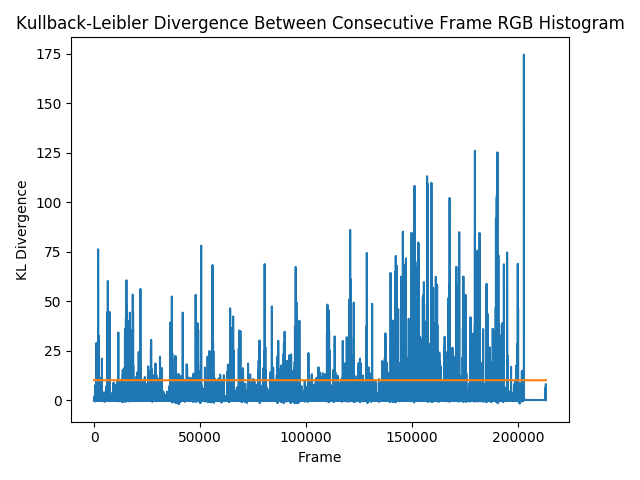
\includegraphics[width=0.70\textwidth]{figures/evaluation/inception_KLdiv_threshold10.png}}
\caption{\label{fig:inception_KLdiv_threshold10}Result of the shot boundary detection algorithm on the Inception movie using the KL Divergence between consecutive frames' RGB histograms.}
\end{figure}

\begin{figure}[h] 
\centerline{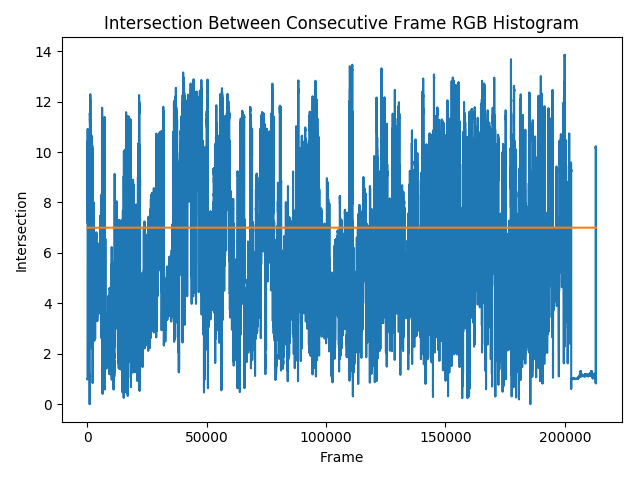
\includegraphics[width=0.70\textwidth]{figures/evaluation/inception_inter_threshold7.png}}
\caption{\label{fig:inception_inter_threshold7}Result of the shot boundary detection algorithm on the Inception movie using the Intersection between consecutive frames' RGB histograms.}
\end{figure}

%%%%%%%%%%%%%%%%%%%%%%%%%%%%%%%%%%%%%%%%%%%%%%%%%%%%%%%%%%%%%%%%%%%%
%%%%%%%%%%%%%%%%%%%%%%%%%%%%%%%%%%%%%%%%%%%%%%%%%%%%%%%%%%%%%%%%%%%%
%%%%%%%%%%%%%%%%%%%%%%%%%%%%%%%%%%%%%%%%%%%%%%%%%%%%%%%%%%%%%%%%%%%%

\section{Summary}

todo